\section{\emph{App Server}}
\label{sec:appserver}
Dieser Abschnitt behandelt das Openshift Projekt \emph{App}-Server, das die gebauten Services beinhaltet. Wenn der Jenkins Service, der im \emph{Build}-Server Projekt enthalten ist am \emph{Cluster} die nötigen Berechtigungen hat, kann die Jenkins Pipeline mit anderen Openshift Projekten interagieren. Da dies in der It\&Tel \emph{Cloud} nicht möglich war, wird zu Demozwecken, der App Service im \emph{Build}-Server Projekt eingespielt. 

\begin{figure}[H]
	\centering
	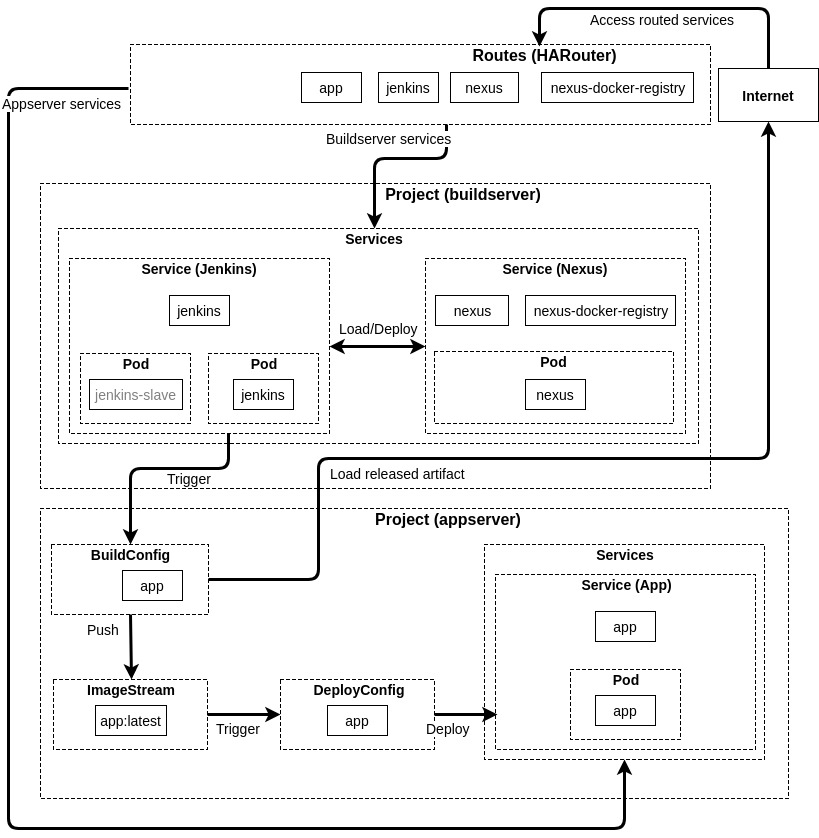
\includegraphics[scale=0.51]{logos/architecture-diagram-appserver.jpg}
	\caption{\emph{App} Server Architektur}
	\label{fig:appserver}
\end{figure}

\subsection{\emph{Update}-Szenarien}
Dieser Abschnitt behandelt die \emph{Update}-Szenarien der Beispielanwendung, die in Jenkins über eine Jenkins Pipeline gebaut wird. Für diese Anwendung gibt es nur ein \emph{Update}-Szenario, nämlich wenn ein Jenkins Pipeline \emph{Build} eine neue Version freigibt, die neu eingespielt werden muss. \\

Die Jenkins Pipeline löst eine \emph{Build}-Konfiguration aus, die das neue Docker Image baut, wobei im Anschluss ein \emph{ImageChagne} Trigger ausgelöst wird, der den Service mit dem neuen Docker Image neu einspielt.
